\chapter{Geometria/Relações (4º Bimestre)}

\section{Resolução de triângulos}

We recall what we saw in el 3º Bimestre de la 8ª série do Ensino Fundamental.
Considere um triângulo retângulo e $\alpha$ a medida de um ângulo
em radianos ($0 \leq \alpha < \frac{\pi}{2}$).

\begin{center}
 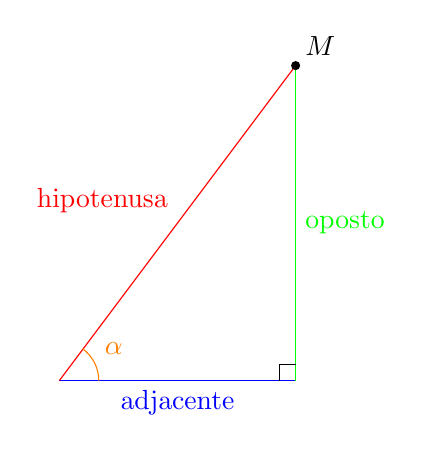
\begin{tikzpicture}
   \draw[color=blue] (0,0) -- (1.5,0)node[below]{adjacente} -- (3,0);
   \draw[color=green] (3,0) -- (3,2)node[right]{oposto} -- (3,4);
   \draw[color=red] (3,4) -- (1.5,2)node[above left]{hipotenusa} -- (0,0);
   \draw (2.8,0) -- (2.8,.2) -- (3,.2);
   \draw[color=orange] (0.5,0) arc(0:25:.5) node[above right]{$\alpha$}
   arc(25:53.13010235415599:.5);
   \draw[fill=black] (3,4) node[above right]{$M$} circle(.05);
 \end{tikzpicture}
\end{center}

Esses ângulos retos e $\alpha$ determinam a classe de semelhança do triângulo
e, portanto, as seguintes frações:

$$
\sin \alpha = \frac{\color{green}{\text{oposto}}}
{\text{\color{red}{\text{hipotenusa}}}}
$$
%%
$$
\cos \alpha = \frac{\color{blue}{\text{adjacente}}}
{\text{\color{red}{\text{hipotenusa}}}}
$$
%%
$$
\tan \alpha = \frac{\color{green}{\text{oposto}}}
{\text{\color{blue}{\text{adjacente}}}}
$$

These relations allow to find all the angles and sides inside a triangle
rectangle from a few parameters. When the triangle is not rectangle,
we can use the Lei dos Cossenos: Sea un triángulo de ángulos
$\alpha, \beta, \gamma$ con lados opuestos a estos
ángulos respectivamente $a,b,c$. Tenemos la relación:

$$a^2 = b^2 + c^2 - {2bc \cos\alpha}$$

\begin{center}
 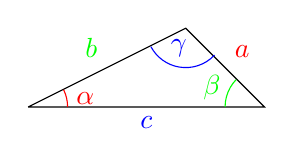
\begin{tikzpicture}
   \draw (0,0) -- (1.5,0) node[below,color=blue]{$c$} -- (3,0) --
   (2.5,.5)node[above right,color=red]{$a$} -- (2,1) --
   (1,.5)node[above left,color=green]{$b$} -- (0,0);

   \draw[color=red](.5,0) arc(0:13:.5) node[right]{$\alpha$}
   arc(13:26:.5);

   \draw[color=green](2.5,0) arc(180:150:.5) node[left]{$\beta$}
   arc(150:136:.5);

   \draw[color=blue](2.365676850809585,0.65900081996875) arc(-43:-100:.5)
   node[above]{$\gamma$} arc(-100:-152:.5);

 \end{tikzpicture}
\end{center}

If we suppose that
$0 < \alpha, \beta, \gamma < \pi$, es decir
$0 < \sin \alpha, \sin \beta, \sin \gamma \leq 1$, we can also use lei dos Senos
%%
$$
\frac{a}{\sin \alpha} = \frac{b}{\sin \beta} =  \frac{c}{\sin \gamma}
$$

\subsection{Exercício 1}

\begin{enumerate}
\item Exprese la ley de cosenos para $\cos \beta$ y $\cos \gamma$.
\item ¿Cómo interpretar el caso $\alpha = \frac{\pi}{2}$?
\item ¿Cómo interpretar el caso $\alpha = \pi$?
\item ¿Cómo interpretar el caso $\alpha = 0$?
\item Suponemos que $b = c$ y $\alpha = \frac{\pi}{3}$. Determine $a$.
\end{enumerate}

\subsection{Exercício 2 (recíproco del teorema de Pitágoras)}

Consideramos un triángulo con las notaciones precedientes.
Muestre que si $a^2 = b^2 + c^2$, el triángulo es rectángulo.

\subsection{Exercício 3}

Consideramos un triángulo con las notaciones precedientes.
Use the lei dos Cossenos to determine una
aproximación de los lados y ángulos si

\begin{enumerate}
  \item Si $a=5\text{cm}$, $b=4\text{cm}$ y $c=7\text{cm}$
  \item Si $\alpha=55°$, $b=8\text{cm}$ y $c=5\text{cm}$
\end{enumerate}

\subsection{Exercício 4 (Lei de Cossenos)}

Consideramos las figuras siguientes donde $x$ es una distancia relativa.

\begin{center}
 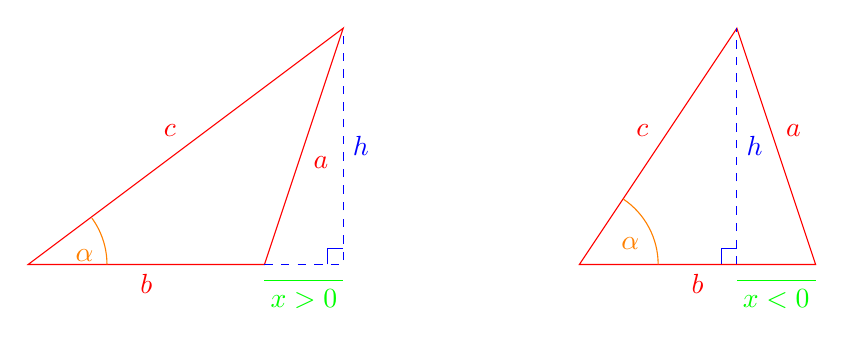
\begin{tikzpicture}
   \draw[color=red]
   (0,0) -- (1.5,0)node[below]{$b$} -- (3,0) --
   (3.5,1.5)node[below right]{$a$}  -- (4,3) --
   (2,1.5) node[above left]{$c$} -- cycle;
   \draw[color=blue,dashed](3,0)--(4,0)--(4,1.5)node[right]{$h$}--(4,3);
   \draw[color=blue](3.8,0)--(3.8,.2)--(4,.2);
   \draw[color=green](3,-.2) -- (3.5,-.2)node[below]{$x>0$} -- (4,-.2);
   \draw[color=orange](1,0) arc(0:18:1)node[below left]{$\alpha$} arc(18:36:1);

   \begin{scope}[shift={(7,0)}]
     \draw[color=red]
     (0,0) -- (1.5,0)node[below]{$b$} -- (3,0) --
     (2.5,1.5)node[above right]{$a$} --
     (2,3) -- (1,1.5)node[above left]{$c$} -- cycle;
     \draw[color=blue,dashed](2,0)--(2,1.5)node[right]{$h$}--(2,3);
     \draw[color=blue](1.8,0)--(1.8,.2)--(2,.2);
     \draw[color=green](3,-.2) -- (2.5,-.2)node[below]{$x<0$} -- (2,-.2);
     \draw[color=orange](1,0) arc(0:28:1)node[below left]{$\alpha$}
     arc(28:56:1);
   \end{scope}
 \end{tikzpicture}
\end{center}

\begin{enumerate}
\item Utilice el teorema de pítagoras en un triángulo rectángulo de hipotenusa
  $a$ para obtener una relación entre $a,h,x$.
\item Utilice el teorema de pítagoras en un triángulo rectángulo de hipotenusa
  $c$ para obtener una relación entre $h,b,x,c$.
\item Muestre $a^2 = c^2 - b^2 - {2bx}$.
\item Exprese $x$ en función de $c, b, \cos{\alpha}$.
\item Deduzca la ley de cosenos.
\end{enumerate}

\subsection{Exercício 5 (triángulos isoceles)}

Consideramos un triángulo con las notaciones precedientes. We also consider
la Lei de Senos:

\begin{enumerate}
  \item Suponemos que $\alpha = \beta$. ¿Que decir de $a,b$?
  \item Suponemos que $a=b$. ¿Que decir de $\alpha, \beta$?
\end{enumerate}

\subsection{Exercício 6}

Consideramos un triángulo con las notaciones precedientes. Using la Lei de
Senos, determine una aproximación de los lados y ángulos si

\begin{enumerate}
  \item Si $b=\text{10cm}$, $\alpha = 20°$ y $\gamma = 55°$
  \item Si $a=\text{10cm}$, $b=\text{8cm}$ y $\alpha = 30°$.
  \item ¿Que decir del caso
    $a=\text{8cm}$, $b=\text{10cm}$ y $\alpha=30°$?
\end{enumerate}

\subsection{Exercício 7 (Lei de Senos)}

Sea $ABC$ un triángulo consideramos su circunferencia circunscrita de centro
$O$ (se puede mostrar que siempre existe y por lo tanto $O$ es la interseción
de las mediatrices de los lados). Sea $D$ tal que $DC$ es un diámetro
y entonces $BCD$ rectángulo en $B$.

\begin{center}
 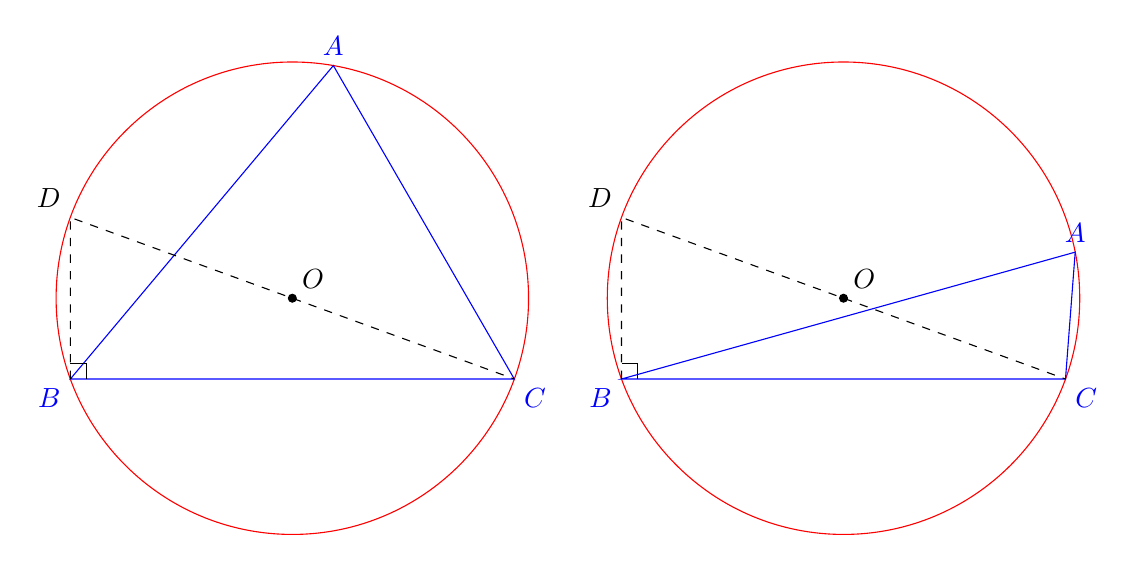
\begin{tikzpicture}
   \draw[color=red] (0,0) circle(3);
   \draw[color=blue]
   (0.52094453300079,2.954423259036624) node[above]{$A$} --
   (-2.819077862357725,-1.026060429977006) node[below left]{$B$} --
   (2.819077862357725,-1.026060429977006) node[below right]{$C$} -- cycle;
   \draw[fill=black] (0,0) node[above right]{$O$} circle(.05);

   \draw[dashed]
   (-2.819077862357725,-1.026060429977006) --
   (-2.819077862357725,1.026060429977006) node[above left]{$D$}--
   (2.819077862357725,-1.026060429977006);
   \draw
   (-2.619077862357725,-1.026060429977006) --
   (-2.619077862357725,-.826060429977006) --
   (-2.819077862357725,-.826060429977006);

   \begin{scope}[shift={(7,0)}]
   \draw[color=red] (0,0) circle(3);
   \draw[color=blue]
   (2.942355841209691,0.5852709660483848) node[above]{$A$} --
   (-2.819077862357725,-1.026060429977006) node[below left]{$B$} --
   (2.819077862357725,-1.026060429977006) node[below right]{$C$} -- cycle;
   \draw[fill=black] (0,0) node[above right]{$O$} circle(.05);

   \draw[dashed]
   (-2.819077862357725,-1.026060429977006) --
   (-2.819077862357725,1.026060429977006) node[above left]{$D$}--
   (2.819077862357725,-1.026060429977006);
   \draw
   (-2.619077862357725,-1.026060429977006) --
   (-2.619077862357725,-.826060429977006) --
   (-2.819077862357725,-.826060429977006);
   \end{scope}
 \end{tikzpicture}
\end{center}

\begin{enumerate}
\item Exprese $\sin \widehat{D}$ en función de $a = BC$ y del radio
  $R = OA = OB = OC = OD$.
\item Show that $\widehat{OBC} = \widehat{OCB}$.
\item Express $\widehat{D}$ in function of $\widehat{OCB}$.
\item Deduce that $2 \widehat{D} = \widehat{BOC}$.
\item Let $E$ be the point diametrically opposite to $A$.
  Show that $2 \widehat{BAE} = \widehat{BOE}$ and
  $2 \widehat{CAE} = \widehat{COE}$.
\item Deduce that $2 \widehat{A} = \widehat{BOC}$.
\item Show that $\frac{a}{\sin \widehat{A}} = 2R$.
\item Deduzca la ley de senos.
\end{enumerate}

\section{Polígonos regulares}

In 3º Bimestre de la 5ª série do Ensino Fundamental we defined polígonos
as a sequence of segmentos
${[A_1,A_2]}, {[A_2, A_3]}, {[A_3, A_4]},\ldots,
{[A_{n-1},A_n]}, {[A_{n},A_1]}$ forming a closed shape.
We also saw
simple/complex, convex/concave, regular polygons as well as various names of
polygons according to the number of sides.
In the 2º Bimestre de la 6ª série do Ensino Fundamental, gave more definitions:
side, vertice, diagonal, Ángulo interior de un polígono simple,
Ángulo exterior de un polígono simple convexo,
centro/Ángulo central/Apotema de un polígono regular.

In this section, we focus on polígonos regulare. Recall that this means that
all angles are equal in measure and all sides have the same length.
We distinguish two kinds of regular polygons: convex (as $A_0A_1A_2A_3A_4$
in the following example)
or star (i.e concave, as $B_0B_1B_2B_3B_4$ in the following example).

\begin{center}
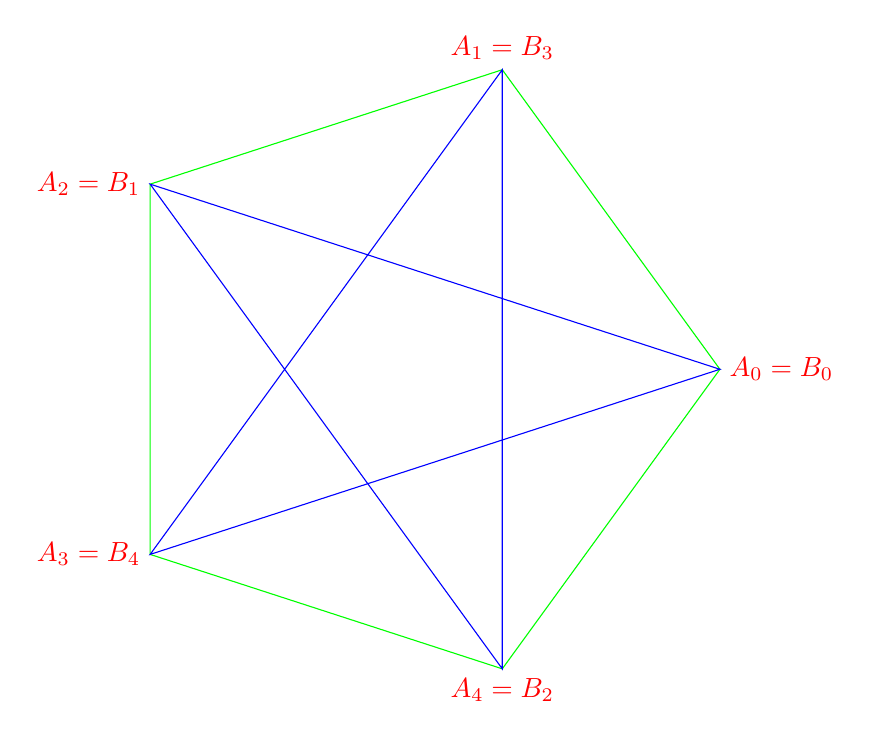
\begin{tikzpicture}
  \draw[color=green]
  (4, 0) --
  (1.23606797749979,3.804226065180614) --
  (-3.236067977499789,2.351141009169893) --
  (-3.236067977499789,-2.351141009169892) --
  (1.23606797749979,-3.804226065180614) --
  cycle;
  \draw[color=blue]
  (4, 0) --
  (-3.236067977499789,2.351141009169893) --
  (1.23606797749979,-3.804226065180614) --
  (1.23606797749979,3.804226065180614) --
  (-3.236067977499789,-2.351141009169892) --
  cycle;

  \draw[color=red]
  (4, 0) node[right] {$A_0=B_0$}
  (1.23606797749979,3.804226065180614) node[above] {$A_1=B_3$}
  (-3.236067977499789,2.351141009169893) node[left] {$A_2=B_1$}
  (-3.236067977499789,-2.351141009169892) node[left] {$A_3=B_4$}
  (1.23606797749979,-3.804226065180614) node[below] {$A_4=B_2$};
\end{tikzpicture}
\end{center}

Note that a star regular polygon is determine by two parameters ${n/m}$ where
$n$ is still the number of sides and $m-1 \geq 1$ indicate the number of
vertices skipped when drawing a side. If we enumerate as
$A_0, A_1, \dots A_{n-1}$
the vertices of the regular convex polygon, then the vertices
of the star regular polygon ${n/m}$ are $B_0, B_2, \dots B_{n-1}$ where
$B_{i} = A_{i \times m \mod n}$ where $i \times m \mod n$ is the remainder of the
Euclidean division of $i \times m$ by $n$.
For example, $m = 2$ in the following pentagram since we skip one vertex each
time. It is easy to verify that $n \geq 5$ and that it is enough (by symmetry)
to consider $m \leq \frac{n}{2}$.
We want all the points of $A_0, A_1, \dots, A_{n-1}$ of the convex polygon
to be reached,
so in particular there should be some $0 \leq i < n$
such that $B_i = A_1$. If $q$ is the
quotient of the previous Euclidean division, we obtain $im = q n + 1$
and so any common divisor $d \geq 1$ of $m$ and $n$ divides
$1 = im  - q n$ that is $d = 1$. Conversely, suppose that the largest common
divisor of $n$ and $m$ is $d = 1$. If $0 \leq i \leq j < n$ satisfy
$B_i = B_j$ then there are $q_1 \leq q_2$ such that
$i m - q_1 n = j m - q_2 n$, that is ${(j - i)} m = {(q_2 - q_1)} n$. Since
$m$ and $n$ don't have any common prime factor $p$ we deduce by comparing the
prime decompositions that $m$ divides $q_2 - q_1$ and so
$j - i = \frac{q_2-q_1}{m} n$ is a multiple of $n$. But this is only possible
if $j - i = 0$ that is $i = j$. Hence $B_0, B_2, \dots B_{n-1}$ is indeed
the enumeration of the $n$ distinct points of the convex polygon.
To summarize, a star regular polygon is defined by numbers ${n/m}$ where
$n \geq 5$ is the number of sides and $1 < m < \frac{n}{2}$ is such that the
largest common divisor of $n$ and $m$ is $1$.

We also recall the specific definitions of regular poligons:
\begin{enumerate}
\item Centro de un polígono regular: es el punto equidistante de todos los vértices y lados.
\item Ángulo central de un polígono regular:
  es el formado por dos segmentos de recta que parten del centro a los extremos
  de un lado.
\item Apotema de un polígono regular: es el segmento que une el centro del polígono con el centro de un lado; es perpendicular a dicho lado.
\item El circumradio de un polígono regular: the length of any segment from
  the center to a vertex of the polygon.
\end{enumerate}

\begin{center}
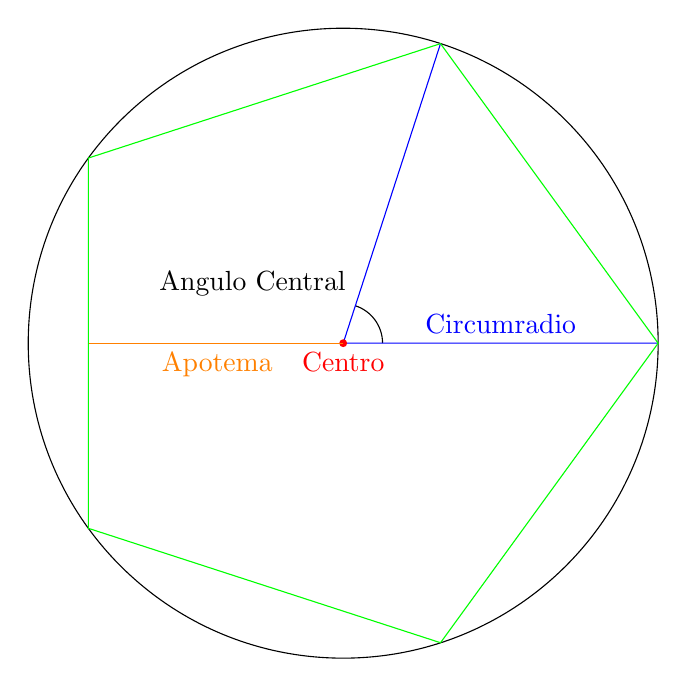
\begin{tikzpicture}
  \draw (0,0) circle(4);
  \draw (.5,0) arc(0:72:.5) node[above left] {Angulo Central};
  \draw (4, 0)[color=blue] -- (2,0) node[above] {Circumradio} -- (0,0) --
  (1.23606797749979,3.804226065180614);
  \fill(0,0) circle(.05)[color=red] node[below] {Centro};
  \draw[color=orange] (0,0) --
  (-1.6,0) node[below]{Apotema} -- (-3.236067977499789,0);

  \draw[color=green]
  (4, 0) --
  (1.23606797749979,3.804226065180614) --
  (-3.236067977499789,2.351141009169893) --
  (-3.236067977499789,-2.351141009169892) --
  (1.23606797749979,-3.804226065180614) --
  cycle;

\end{tikzpicture}
\end{center}

We note that the polígono is circunscrição to the circunferência
of center the center of the polígono and radius the apotema. It is inscrição in
the circunferência of center the center of the polígono and radius a
Circumradio:

\begin{center}
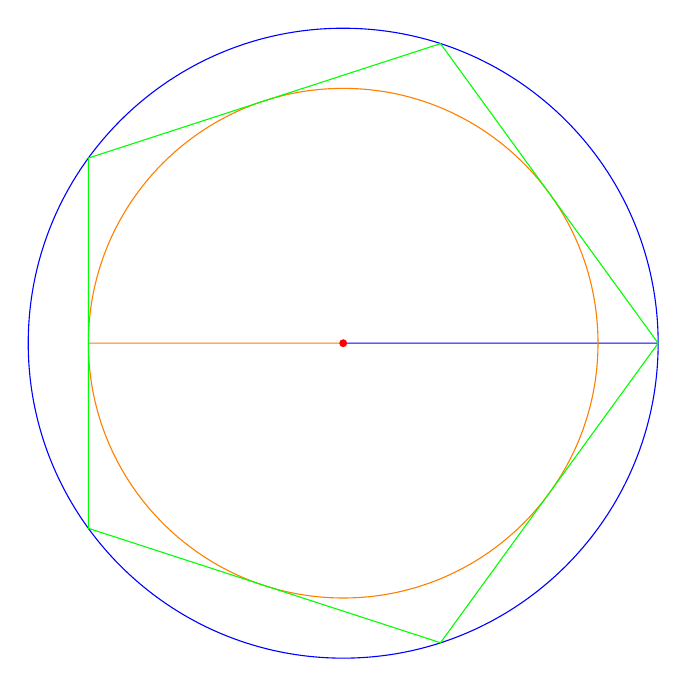
\begin{tikzpicture}
  \draw[color=blue] (4,0) -- (0,0) circle(4);
  \draw[color=orange](-3.236067977499789,0) -- (0,0) circle(3.236067977499789);
  \fill(0,0) circle(.05)[color=red];
  \draw[color=green]
  (4, 0) --
  (1.23606797749979,3.804226065180614) --
  (-3.236067977499789,2.351141009169893) --
  (-3.236067977499789,-2.351141009169892) --
  (1.23606797749979,-3.804226065180614) --
  cycle;
\end{tikzpicture}
\end{center}

In the 2º Bimestre de la 6ª série do Ensino Fundamental, we saw various
ways to construct regular convex polygons with 2, 4, 5, 6, 8, 10, 12, 15, 16
sides using regla y compaso. We can also use a transferidor, to draw other
regular polygons from the values of their central or interior angle.
We recall that for a regular convex polygon the central angle has measure
$\frac{360°}{n}$ and the interior angle $180° \times \frac{n-2}{n}$.

By repeating the same pattern of one or more convex regular polygons, we can
cover the plan. A necessary condition for such pavimentação to be possible is
that at any vertex shared by $N$ regular polygons with $n_1, n_2, \dots, n_N$
sides, the interior angles at that vertex sum up to 360°, that is
$\sum_{i=1}^N (180° \times \frac{n_i-2}{n_i}) = 360°$.
For example, the case $N=3$ and $n_1=n_2=n_3=6$ correspond to an hexagonal
pavimentação:

\begin{center}
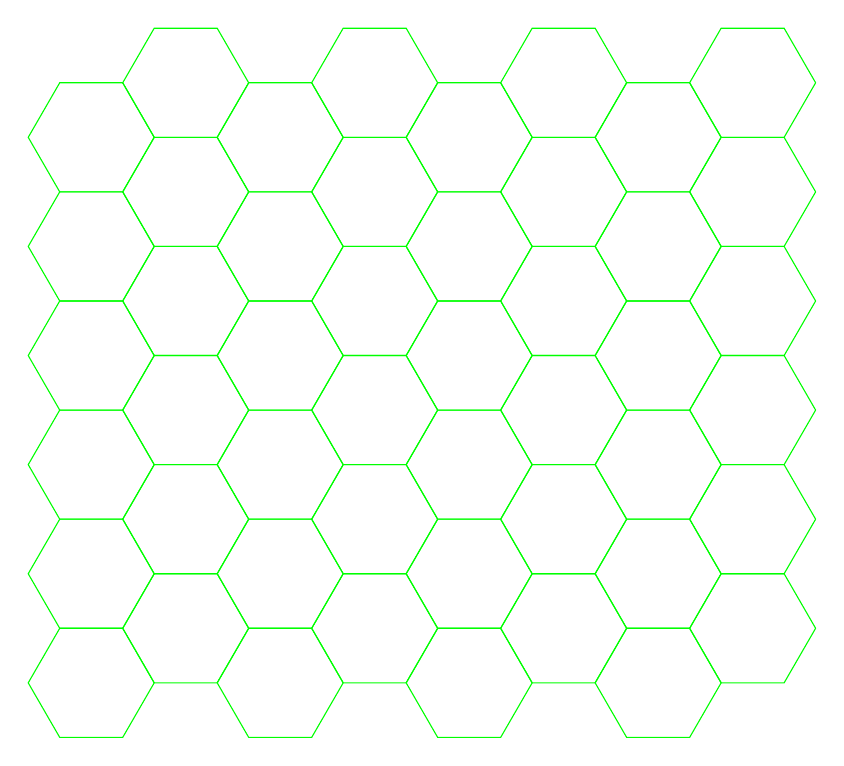
\begin{tikzpicture}[scale=.2]
  \foreach \i in {0,...,3} {
    \foreach \j in {0,...,5} {
      \begin{scope}[shift={(\i*12,\j*3.464101615137754*2)}]
        \draw (4,0) -- (2,3.464101615137754) -- (-2,3.464101615137754) --
        (-4,0) -- (-2,-3.464101615137754) -- (2,-3.464101615137754) -- (4,0)
              [color=green];
        \begin{scope}[shift={(6,3.464101615137754)}]
        \draw (4,0) -- (2,3.464101615137754) -- (-2,3.464101615137754) --
        (-4,0) -- (-2,-3.464101615137754) -- (2,-3.464101615137754) -- (4,0)
              [color=green];
        \end{scope}
      \end{scope}
    }
  }
\end{tikzpicture}
\end{center}

\subsection{Exercício 8}

In this exercise, we only use regla y compaso.

\begin{enumerate}
\item Fix a point $O$ and draw a circumference
  $\mathcal C$ of radius $R=4\text{cm}$.
\item Draw a line ${\mathcal D}_1$ passing by $O$. It intersects $\mathcal C$
  at points $A_0, A_2$.
\item Construct a line ${\mathcal D}_2$ orthogonal to ${\mathcal D}_1$ and
  passing by $O$. It intersects $\mathcal C$ at points $A_1, A_3$
  such that $A_0,A_1,A_2,A_3$ are enumerated clockwise.
\item What is the convex regular polygon $A_0A_1A_2A_3$?
  Can we obtain a star regular polygons from its vertices?
\item Draw the four lines passing by $A_i$ and orthogonal to $(OA_i)$ for
  $i = 1, 2, 3, 4$. These lines intersects at points
  $B_1, B_2, B_3, B_4$. What is the convex regular polygon made by these points?
\item Construct a regular hexagon $C_0C_1C_2C_3C_4C_5$ inscribed in $\mathcal C$.
  Can we obtain a star regular polygons from its vertices?
\item What is the triangle $C_0C_2C_4$?
  Can we obtain a star regular polygons from its vertices?
\item The mediatriz of $[C_0C_1]$ intersects $\mathcal C$ at point $X$.
  Then the line passing by $X$ and orthogonal to $(OX)$ intersects
  $(OC_0)$ at $Y$. Draw a regular convex hexagon inscribed in the circumference
  of center $O$ and radius $OY$. What can you say about this hexagon?
\item Draw the three lines passing by $C_i$ and orthogonal to $(OC_i)$ for
  $i = 1, 3, 5$. They intersect at three points. What can you say about the
  triangle obtained?
\item Comming back to the points $A_0,A_1,A_2,A_3$ we note that the mediatrices
  of $[A_0A_1]$ and $[A_1A_2]$ intersect $\mathcal C$ at four more points.
  Draw the corresponding regular convex octogon $D_0D_1D_2D_3D_4D_5D_6D_7$.
\item Show that we can obtain only one star regular polygon from the
  points $D_0, D_1, D_2, D_3, D_4, D_5, D_6, D_7$ and draw it.
\end{enumerate}

\subsection{Exercício 9}

We fix a point $O$ and consider the circumference $\mathcal C$ of radius
$R=4\text{cm}$.

\begin{enumerate}
\item What is the measure $\alpha$ of the internal angle of a regular heptagon
  ($7$-gono)?
\item Let $A_0$ be a point on $\mathcal C$. Use the transferidor to construct
  a point $A_1$ on $\mathcal C$ such that
  $\widehat{OA_0A_1} = \frac{\alpha}{2}$. Construct a regular heptagon
  $A_0A_1A_2A_3A_4A_5A_6$ inscribed in $\mathcal C$.
\item What is the measure $\beta$ of the central angle of a regular heptagon
  ($7$-gono)?
\item Let $\mathcal D$ be the line passing by $A_0$ and orthogonal to
  $(OA_0)$. Use the transferidor to construct
  two points $B_0, B_1$ on $\mathcal D$ such that
  $\widehat{OA_0B_0} = \widehat{OA_0B_1} = \frac{\beta}{2}$.
  Construct a regular heptagon
  $B_0B_1B_2B_3B_4B_5B_6$ circumbscribed in $\mathcal C$.
\item Calculate the length of $A_0A_1$ and $B_0B_1$ and verify your result.
  Deduce an alternative way to draw the inscribed and circumscribed heptagons
  using graduated ruler and compass.
\item Show that we can obtain exactly two star regular polygon from the
  points $A_0, A_1, A_2, A_3, A_4, A_5, A_6$ and draw them.
\end{enumerate}

\subsection{Exercício 10}

\begin{enumerate}
\item Suppose that we have a pavimentação with regular polygons.
  Show that if at a vertex is surrounded by $N$ polygons with
  $n_1, n_2, \dots, n_N$ sides then
  $$\sum_{i}^N \frac{1}{n_i} = \frac{N-2}{2}$$
  and deduce that $N \geq 3$.
\item What are the values of $N$ and $n_1, n_2, \dots, n_N$ for the standard
  pavimentação with squares of same size?
\item Prove that $\sum_{i}^N \frac{1}{n_i} \leq \frac{N}{3}$ and deduce that
  $N \leq 6$.
\item Suppose $N=6$ and $n_6 \geq 4$. Prove that
  $\sum_{i}^{N-1} \frac{1}{n_i} \leq \frac{5}{3} < \frac{7}{4} \leq
  \frac{N-2}{2} - \frac{1}{n_N}$.
\item What is the only possible case for $N=6$?
\item Draw a pavimentação with $N=6$ regular polygons at each vertex.
\item In the previous case, the six equilateral triangles around a vertex can
  be ``merged'' into one regular hexagon. By building 1, 2, or 3 hexagons around
  a vertex deduce some cases for $N=3$, $N=4$ or $N=5$.
\item Find pavimentaçãos where the previous cases happen at each vertex.
\item Determine the values of $N$ and $n_1, n_2, \dots, n_N$ for the following
  pavimentação:

  \begin{center}
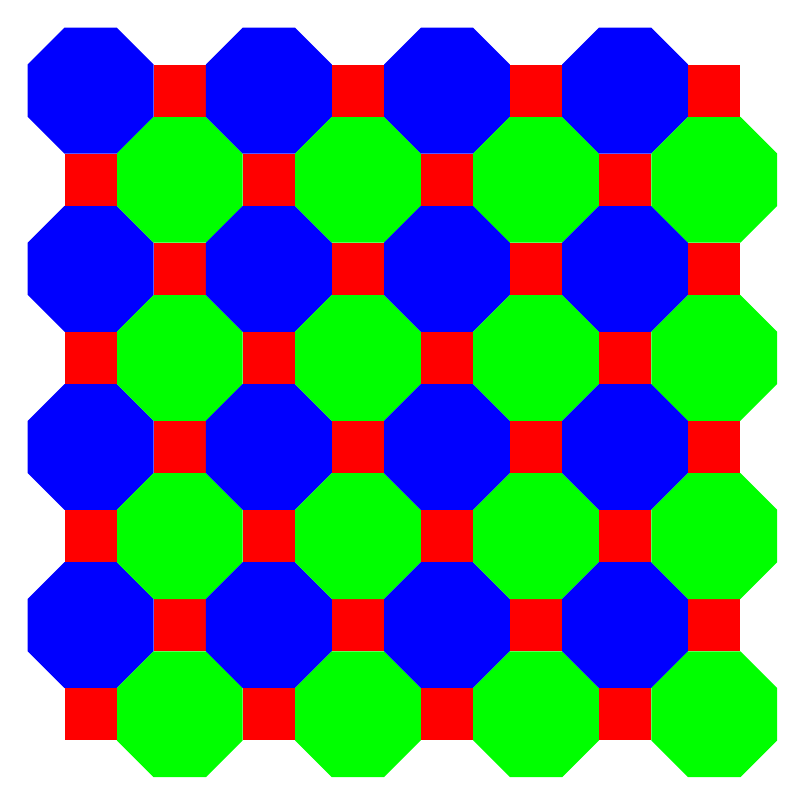
\begin{tikzpicture}[scale=.2]
  \foreach \i in {0,...,3} {
    \foreach \j in {0,...,3} {
      \begin{scope}[shift={(\i*11.31370849898476,\j*11.31370849898476)}]
  \fill[color=blue]
  (4, -1.65685424949238) -- (4, 1.65685424949238) --
  (1.65685424949238, 4) -- (-1.65685424949238, 4) --
  (-4, 1.65685424949238) -- (-4,-1.65685424949238) --
  (-1.65685424949238, -4) -- (1.65685424949238, -4) -- cycle;
  \begin{scope}[shift={(5.65685424949238, -5.65685424949238)}]
  \fill[color=green]
  (4, -1.65685424949238) -- (4, 1.65685424949238) --
  (1.65685424949238, 4) -- (-1.65685424949238, 4) --
  (-4, 1.65685424949238) -- (-4,-1.65685424949238) --
  (-1.65685424949238, -4) -- (1.65685424949238, -4) -- cycle;
  \end{scope}
  \begin{scope}[shift={(5.65685424949238, 0)}]
  \fill[color=red]
  (1.65685424949238,1.65685424949238) --
  (-1.65685424949238,1.65685424949238) --
  (-1.65685424949238,-1.65685424949238) --
  (1.65685424949238,-1.65685424949238) -- cycle;
  \end{scope}
  \begin{scope}[shift={(0,-5.65685424949238)}]
  \fill[color=red]
  (1.65685424949238,1.65685424949238) --
  (-1.65685424949238,1.65685424949238) --
  (-1.65685424949238,-1.65685424949238) --
  (1.65685424949238,-1.65685424949238) -- cycle;
  \end{scope}
      \end{scope}
    }
  }
\end{tikzpicture}
\end{center}

\item
  Verify that $N=3$, $n_1=3$, $n_2=10$ and $n_3=15$ satisfies
  $\sum_{i}^N \frac{1}{n_i} = \frac{N-2}{2}$.
  Can we find a pavimentação that has these parameters at each vertex?
\end{enumerate}

\subsection{Exercício 10}

\begin{enumerate}
\item As discussed in the course summary, we must have
  $\sum_{i=1}^N (180° \times \frac{n_i-2}{n_i}) = 360°$. After simplification,
  we obtain the desired formula.
  Then $\frac{N-2}{2} = \sum_{i}^N \frac{1}{n_i} > 0$ implies
  $N > 2$.
\item $N=4$ and $n_1=n_2=n_3=n_4=4$. We verify
  $N \times \frac{1}{4} = 1 = \frac{N-2}{2}$.
\item Each polygon has at least 3 sides so $n_i \geq 3$,
  $\frac{1}{n_i} \leq \frac{1}{3}$ and
  $\frac{N-2}{2} = \sum_{i}^N \frac{1}{n_i} \leq \frac{N}{3}$.
  So $3N - 6 \leq 2N$ and $N \leq 6$.
\item As above, $\sum_{i}^{N-1} \frac{1}{n_i} \leq \frac{N-1}{3} = \frac{5}{3}$.
  If $n_6 \geq 4$ then $\frac{1}{n_6} \leq \frac{1}{4}$ and
  $-\frac{1}{n_6} \geq -\frac{1}{4}$.
  Hence $\frac{N-2}{2} -\frac{1}{n_6} \geq 2 - \frac{1}{4} = \frac{7}{4}$.
  Now $\frac{5}{3} < \frac{7}{4}$ so the equality
  $\frac{N-2}{2} = \sum_{i}^N \frac{1}{n_i}$ can not happen.
\item By the previous question, the only possibility is
  $n_1=n_2=n_3=n_4=n_5=n_6=3$. We verify that indeed,
  $\sum_{i=1}^6 \frac{1}{n_i} = \frac{6}{3} = 2 = \frac{6-2}{2}$.
\item A pavimentação made of equilateral triangles:

  \begin{center}
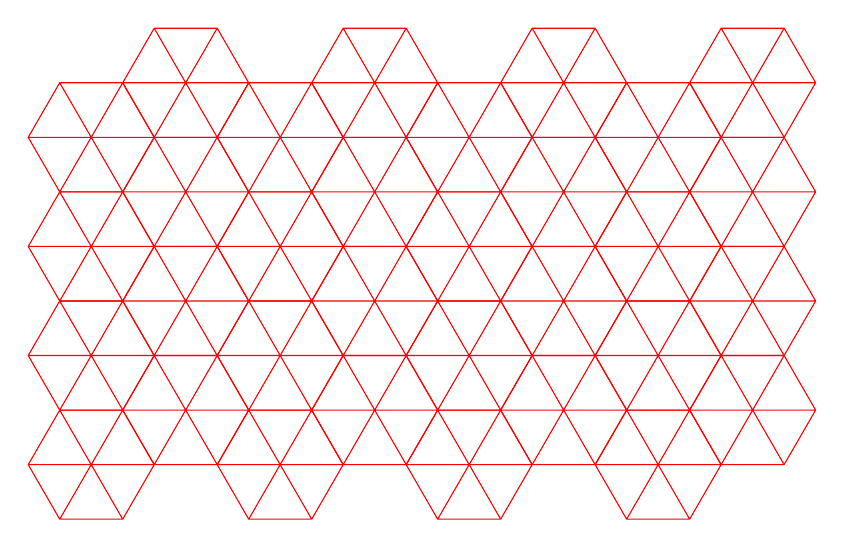
\begin{tikzpicture}[scale=.2]
  \foreach \i in {0,...,3} {
    \foreach \j in {0,...,3} {
      \begin{scope}[shift={(\i*12,\j*3.464101615137754*2)}]
        \draw (4,0) -- (2,3.464101615137754) -- (-2,3.464101615137754) --
        (-4,0) -- (-2,-3.464101615137754) -- (2,-3.464101615137754) -- (4,0)
        (4,0) -- (0,0)
        (2,3.464101615137754) -- (0,0)
        (-2,3.464101615137754) -- (0,0)
        (-4,0) -- (0,0)
        (-2,-3.464101615137754) -- (0,0)
        (2,-3.464101615137754) -- (0,0)
              [color=red];
        \begin{scope}[shift={(6,3.464101615137754)}]
        \draw (4,0) -- (2,3.464101615137754) -- (-2,3.464101615137754) --
        (-4,0) -- (-2,-3.464101615137754) -- (2,-3.464101615137754) -- (4,0)
        (4,0) -- (0,0)
        (2,3.464101615137754) -- (0,0)
        (-2,3.464101615137754) -- (0,0)
        (-4,0) -- (0,0)
        (-2,-3.464101615137754) -- (0,0)
        (2,-3.464101615137754) -- (0,0)
              [color=red];
        \end{scope}
      \end{scope}
    }
  }
\end{tikzpicture}
\end{center}
\item If we build three hexagons around a vertex, we obtain the case
  $N=3$ and $n_1=n_2=n_3=6$.
  If we build only two hexagons and keep two triangles around the vertex we get
  $N=2+2=4$, $n_1=n_2=6$ and $n_3=n_4=3$.
  If we build only one hexagon and keep four triangles around the vertex we get
  $N=1+4=5$, $n_1=6$ and $n_2=n_3=n_4=n_5=3$.
\item We already met $N=3$ and $n_1=n_2=n_3=6$ for the hexagonal pavimentação.
  For the case $N=4$, $n_1=n_2=6$ and $n_3=n_4=3$ consider:

  \begin{center}
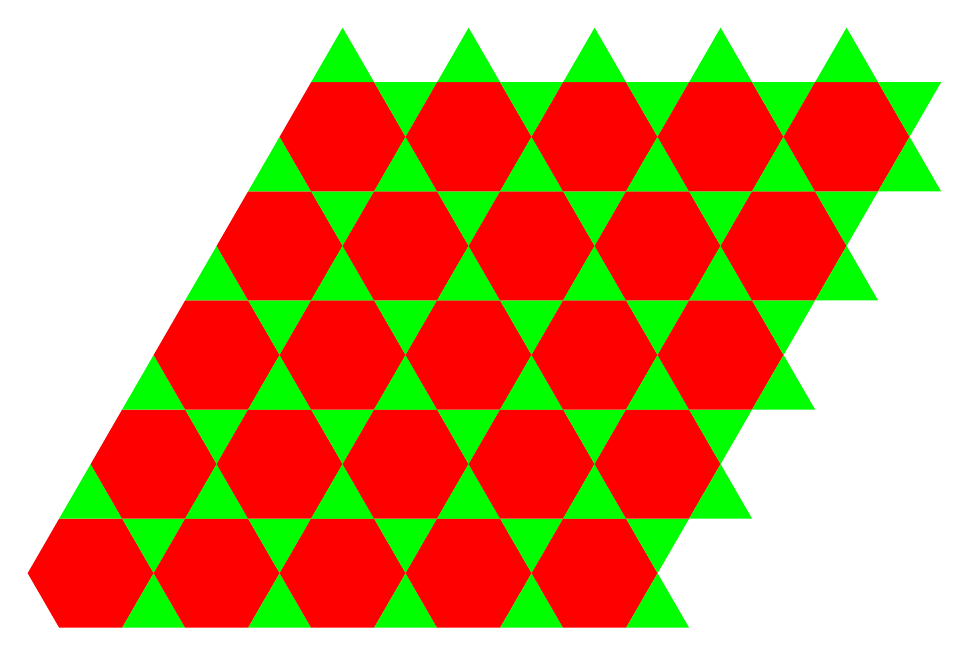
\begin{tikzpicture}[scale=.2]
  \foreach \i in {0,...,4} {
  \foreach \j in {0,...,4} {
    \begin{scope}[shift={(\i*8 + \j*4,\j*2*3.464101615137754)}]
   \fill[color=red] (4,0) -- (2,3.464101615137754) -- (-2,3.464101615137754) --
  (-4,0) -- (-2,-3.464101615137754) -- (2,-3.464101615137754) -- (4,0);
  \begin{scope}[shift={(2,-3.464101615137754)}]
  \fill[color=green] (4,0) -- (0,0) -- (2,3.464101615137754);
  \end{scope}
  \begin{scope}[shift={(-2,3.464101615137754)}]
  \fill[color=green] (4,0) -- (0,0) -- (2,3.464101615137754);
  \end{scope}
  \begin{scope}[shift={(4,0)}]
  \fill[color=green] (-2,3.464101615137754) -- (0,0) -- (2,3.464101615137754);
  \end{scope}
  \end{scope}
  }
  }
\end{tikzpicture}
\end{center}
  For the case $N=5$, $n_1=6$ and $n_2=n_3=n_4=n_5=3$, consider:
  \begin{center}
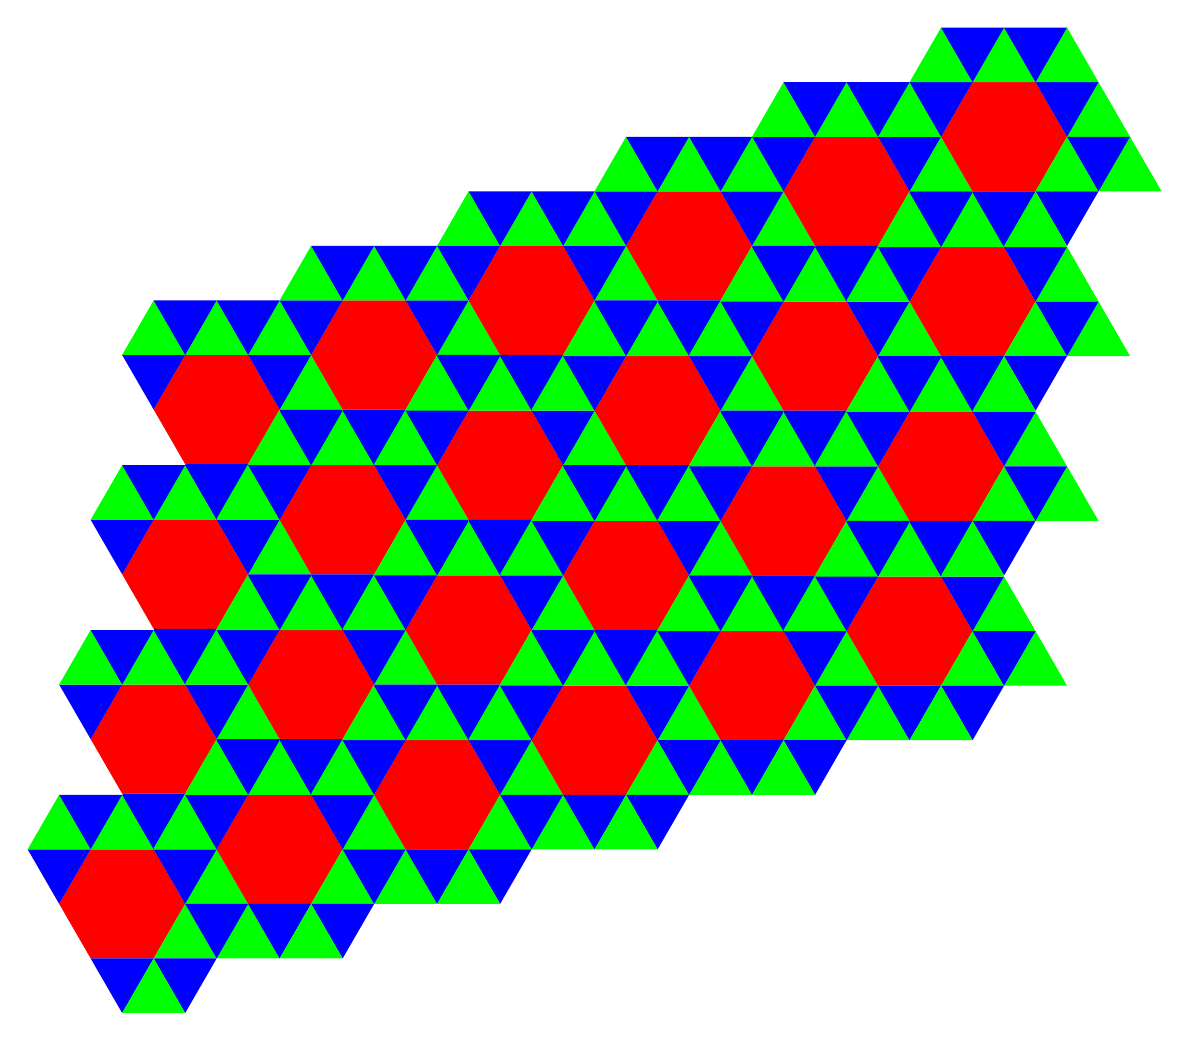
\begin{tikzpicture}[scale=.2]
 \foreach \i in {0,...,5} {
  \foreach \j in {0,...,3} {
   \begin{scope}[shift={(\i*10+2*\j,\i*3.464101615137754+\j*10.46410161513775)}]
  \fill[color=red] (4,0) -- (2,3.464101615137754) -- (-2,3.464101615137754) --
  (-4,0) -- (-2,-3.464101615137754) -- (2,-3.464101615137754) -- (4,0);
   \begin{scope}[shift={(2,-3.464101615137754)}]
  \fill[color=green] (4,0) -- (0,0) -- (2,3.464101615137754) -- cycle;
  \end{scope}
  \begin{scope}[shift={(4,0)}]
  \fill[color=green] (4,0) -- (0,0) -- (2,3.464101615137754) --cycle;
  \end{scope}
  \begin{scope}[shift={(6,-3.464101615137754)}]
  \fill[color=green] (4,0) -- (0,0) -- (2,3.464101615137754) --cycle;
  \end{scope}
  \begin{scope}[shift={(4,0)}]
  \fill[color=blue] (-2,3.464101615137754) -- (0,0) -- (2,3.464101615137754);
  \end{scope}
  \begin{scope}[shift={(-4,0)}]
  \fill[color=blue] (-2,3.464101615137754) -- (0,0) -- (2,3.464101615137754);
  \end{scope}
  \begin{scope}[shift={(6,-3.464101615137754)}]
  \fill[color=blue] (-2,3.464101615137754) -- (0,0) -- (2,3.464101615137754);
  \end{scope}
  \begin{scope}[shift={(0,-6.928203230275508)}]
  \fill[color=blue] (-2,3.464101615137754) -- (0,0) -- (2,3.464101615137754);
  \end{scope}
  \begin{scope}[shift={(4,-6.928203230275508)}]
  \fill[color=blue] (-2,3.464101615137754) -- (0,0) -- (2,3.464101615137754);
  \end{scope}
  \begin{scope}[shift={(0,-6.928203230275508)}]
  \fill[color=green] (4,0) -- (0,0) -- (2,3.464101615137754) -- cycle;
  \end{scope}
  \begin{scope}[shift={(2,3.464101615137754)}]
  \fill[color=green] (4,0) -- (0,0) -- (2,3.464101615137754) -- cycle;
  \end{scope}
  \begin{scope}[shift={(-2,3.464101615137754)}]
  \fill[color=green] (4,0) -- (0,0) -- (2,3.464101615137754) -- cycle;
  \end{scope}
  \begin{scope}[shift={(-6,3.464101615137754)}]
  \fill[color=green] (4,0) -- (0,0) -- (2,3.464101615137754) -- cycle;
  \end{scope}
  \begin{scope}[shift={(2,3.464101615137754)}]
  \fill[color=blue] (-2,3.464101615137754) -- (0,0) -- (2,3.464101615137754);
  \end{scope}
  \begin{scope}[shift={(-2,3.464101615137754)}]
  \fill[color=blue] (-2,3.464101615137754) -- (0,0) -- (2,3.464101615137754);
  \end{scope}
  \end{scope}
  }
  }
\end{tikzpicture}

\end{center}

\item At each vertex, there is one square and two octogons so
  $N=3$, $n_1=n_2=8$ and $n_3=4$ and we have indeed
  $\frac{2}{8} + \frac{1}{4} = \frac{1}{2} = \frac{3-2}{2}$

\item
  We have indeed $\frac{1}{3} + \frac{1}{10} + \frac{1}{15} =
  \frac{1}{2} = \frac{3-2}{2}$.
  Suppose we have a pavimentação that has these parameters at each vertex and
  consider one equilateral triangle. At each vertex of the triangle,
  there must be two other polygons sharing the same vertex
  (a decagon and a pentadecagon). However, it is not possible to place
  three polygons around the triangle such that this property is satisfied.
  So such a pavimentação does not exist.
\end{enumerate}

\section{Solução do Exercícios}

\subsection{Exercício 1}

\begin{enumerate}
\item
  $$b^2 = c^2 + a^2 - {2ca \cos \beta}$$
  $$c^2 = a^2 + b^2 - {2ab \cos \gamma}$$

\item Si $\alpha = \frac{\pi}{2}$, $\cos \alpha = 0$ y el triángulo es
  rectángulo. Obtenemos el teorema de pítagoras: $a^2 = b^2+c^2$.
\item Si $\alpha = \pi$, $\cos \alpha = -1$ y el vértice corespondiente
  al ángulo $\alpha$ apartene al lado opuesto. Obtenemos
  $a^2 = b^2 + c^2 + {2bc} = {b+c}^2$ es decir $a = b + c$.
\item Si $\alpha = 0$, $\cos \alpha = 1$ y los lados adyacentes al ángulo
  $\alpha$ son sobre la misma semirecta. Obentemos
  $a^2 = b^2 + c^2 - {2bc} = {b-c}^2$ es decir $a = b - c$ (si $b \geq c$) o
  $a = c - b$ (si $c \geq b$).
\item Si $b = c$ y $\alpha = \frac{\pi}{3}$, obtenemos
  $a^2 = b^2 + b^2 - {2bc\frac{1}{2}} = b^2$ es decir $a=b=c$. En efecto
  eso coresponde a un triángulo equilatero.

\end{enumerate}

\subsection{Exercício 2 (recíproco del teorema de Pitágoras)}

$2bc \cos \alpha = a^2 - b^2 - c^2 = 0$. Porque $b, c > 0$ y
$0 \leq \alpha \leq \pi$, obtenemos $\alpha = \frac{\pi}{2}$ y el triángulo
es rectángulo.

\subsection{Exercício 3}

\begin{enumerate}
  \item
    $\alpha =
    \arccos \left( \frac{a^2-b^2-c^2}{-2bc} \right) \approx
    44°$,
    $\beta =
    \arccos \left( \frac{b^2-a^2-c^2}{-2ac} \right) \approx 34°$ y
    $\gamma =
    \arccos \left( \frac{c^2-a^2-b^2}{-2ab} \right) \approx 102°$.
  \item
    $a = \sqrt{b^2 + c^2 - {2bc \cos \alpha}} \approx
    6.57 \text{cm}$ entonces
    $\beta =
    \arccos \left( \frac{b^2-a^2-c^2}{-2ac} \right) \approx 86°$ y
    $\gamma =
    \arccos \left( \frac{c^2-a^2-b^2}{-2ab} \right) \approx 39°$.
\end{enumerate}

\subsection{Exercício 4 (ley de cosenos)}

\begin{enumerate}
\item $a^2 = h^2 + x^2$
\item $c^2 = h^2 + \left(b+x\right)^2$
\item Desde las relaciones precedientes, obtenemos
  $c^2 = h^2 + x^2 + {2bx} + b^2 = a^2 + {2bx} + b^2$ es decir
  $a^2 = c^2 - b^2 - {2bx}$.
\item $\cos \alpha = \frac{b+x}{c}$ entonces
  $x = {c \cos \alpha} - b$.
\item $a^2 = c^2 - b^2 - {2bx} =
  c^2 - b^2 - {2b \left( {c \cos \alpha} - b \right)} =
  c^2 - b^2 - {bc\cos \alpha} + 2b^2$ y finalmente
  $$a^2 = b^2 + c^2 - {2bc \cos\alpha}$$
\end{enumerate}

\subsection{Exercício 5 (triángulos isoceles)}

\begin{enumerate}
  \item Si $\alpha=\beta$, $\sin \alpha = \sin \beta$ y
    entonces $a=b$.
  \item Si $a=b$, $\sin \alpha = \sin \beta$ es decir
    $\alpha = \beta$ o $\alpha = \pi - \beta$.
    Pero $\gamma = \pi - \alpha - \beta \neq 0$ y entonces $\alpha = \beta$.
\end{enumerate}

\subsection{Exercício 6}

\begin{enumerate}
\item $\beta = 180° - \alpha - \gamma = 105°$. Entonces
$a = \frac{b}{\sin \beta} \sin \alpha \approx
3.54 \text{cm}$ y
$c = \frac{b}{\sin \beta} \sin \gamma \approx 8.48 \text{cm}$

\item $\sin \beta = \frac{\sin \alpha}{a} \times b$
  entonces $\beta = \theta$ (y $\gamma = \pi - \alpha - \theta$) o
  $\beta = \pi - \theta$ (y $\gamma = \theta - \alpha$) donde
  $\theta = \arcsin \left(\frac{\sin \alpha}{a} \times b\right)$.
  Pero $\theta \approx 24° < 30° = \alpha$ entonces sólo el primer caso
  es posible: $\beta \approx 24°$, $\gamma \approx 126°$.
  Obtenemos
    $c = \sqrt{a^2 + b^2 - {2ab \cos \gamma}} \approx 16.1\text{cm}$.

\item Ahora obtenemos $\theta \approx 39° > 30° = \alpha$ y entonces
  existen dos triángulos congruentes que satisfacen estas condiciones.

\end{enumerate}

\subsection{Exercício 7 (ley de senos)}

\begin{enumerate}
\item $\sin \widehat{D} = \frac{a}{2R}$.
\item $OB = OC$ is isosceles in $O$ so $\widehat{ABC} = \widehat{ACB}$
\item $\widehat{D} = 90° - \widehat{OCB}$.
\item Deduce that $2 \widehat{D} = 180° - 2 \widehat{OCB} = \widehat{BOC}$.
\item This is exactly the same proof since $[AE]$ is a diameter.
\item
  If $\widehat{A} = \widehat{BAE} + \widehat{CAE}$
  then $\widehat{BOC} = \widehat{BOE} + \widehat{COE} =
  2\widehat{BAE} + 2\widehat{CAE} = 2\widehat{A}$.
  We have a similar proof if
  $\widehat{A}$ is instead expressed as a difference of
  $\widehat{BAE}$ and $\widehat{CAE}$.
\item
  We have $\widehat{A} = \widehat{D}$ so
  $\frac{a}{\sin \widehat{A}} = \frac{a}{\sin \widehat{D}} = 2R$.
\item De la misma manera, podemos monstrar que
  $\frac{b}{\sin \widehat{B}} = 2R$ ($b = AC$) y
  $\frac{c}{\sin \widehat{C}} = 2R$ ($c = AB$). Finalmente
%%
$$
\frac{a}{\sin \widehat{A}} = \frac{b}{\sin \widehat{B}} =
\frac{c}{\sin \widehat{C}} = 2R
$$

\end{enumerate}

\subsection{Exercício 8}

Constructions in this exercise are similar to what we saw in the 2º Bimestre de
la 6ª série do Ensino Fundamental, so we won't give the details.

\begin{enumerate}
\item /
\item /
\item /
\item It is a regular convex $4$-gon (square) inscribed in $\mathcal C$.
  We can not find a star
  polygon ${n/m}$ with $n=4$ otherwise $1 < m < \frac{4}{2}=2$.
\item It is a regular convex $4$-gon (square) circumscribed to $\mathcal C$.
\item For the construction, we use $C_0C_1 = R = 4\text{cm}$.
  We can not find a star
  polygon ${n/m}$ with $n=6$ otherwise
  $1 < m < \frac{6}{2}=3$ implies $m = 2$ and $2 > 1$ would be a common
  divisor of $m,n$.
\item This is a regular $3$-gon (equilateral triangle) inscribed in
  $\mathcal C$.
  We can not find a star
  polygon ${n/m}$ with $n=3$ otherwise $1 < m < \frac{3}{2} < 2$.
\item It is circumscribed to $\mathcal C$.
\item This is a regular $3$-gon (equilateral triangle) circumbscribed to
  $\mathcal C$.
\item /
\item For $n=8$, a regular star polygon ${n/m}$ satisfies
  $1 < m < \frac{8}{2} = 4$ so $m=2$ or $m=3$. But only $m=3$ satisfies the
  condition that it does not have any divisor $d > 1$ common with $n$.
  Using the previous scheman we obtained the star polygon
  $D_0D_3D_6D_1D_4D_7D_2D_5$ drawn in red.
  \begin{center}
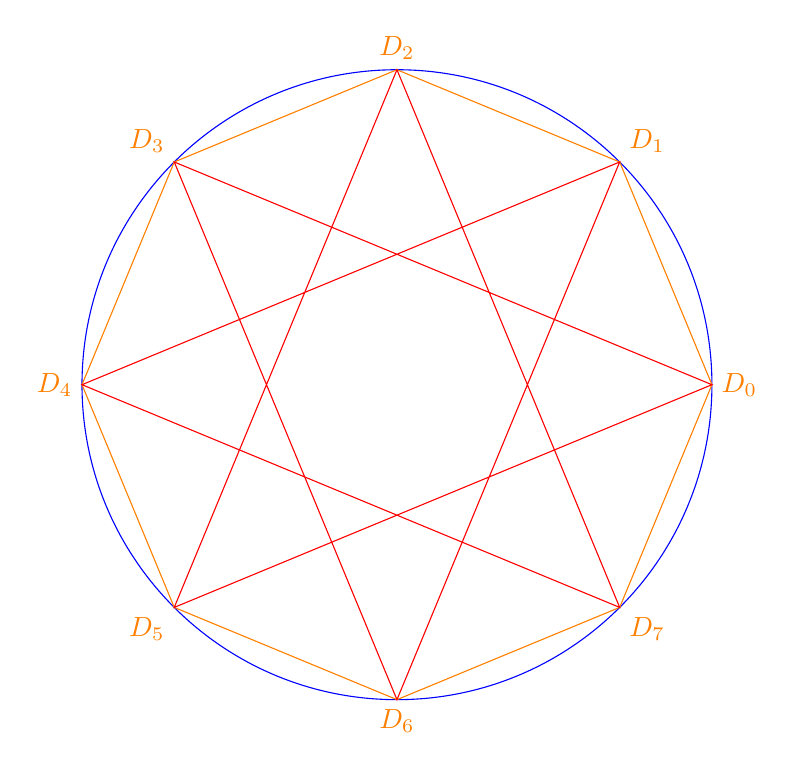
\begin{tikzpicture}
  \draw[color=blue] (0,0) circle(4);
  \draw[color=orange]
  (4, 0) node[right] {$D_0$} --
  (2.82842712474619,2.82842712474619) node[above right] {$D_1$}--
  (0, 4) node[above] {$D_2$} --
  (-2.82842712474619,2.82842712474619) node[above left] {$D_3$} --
  (-4,0) node[left] {$D_4$} --
  (-2.82842712474619,-2.82842712474619) node[below left] {$D_5$} --
  (0,-4) node[below] {$D_6$} --
  (2.82842712474619,-2.82842712474619) node[below right] {$D_7$} --
  cycle;

  \draw[color=red]
  (4, 0) --
  (-2.82842712474619,2.82842712474619) --
  (0,-4) --
  (2.82842712474619,2.82842712474619) --
  (-4,0) --
  (2.82842712474619,-2.82842712474619) --
  (0, 4) --
  (-2.82842712474619,-2.82842712474619) --
  cycle;
\end{tikzpicture}
\end{center}
\end{enumerate}

\subsection{Exercício 9}

\begin{enumerate}
\item $\alpha = 180° \frac{7-2}{7} = \frac{900°}{7} \approx 128.57°$
\item We obtain:
    \begin{center}
    \begin{tikzpicture}
  \draw[color=blue] (0,0) node[above]{$O$} circle(4);
  \draw[color=green] (0,0) -- (3.5,0) node[above]{$\frac{\alpha}{2}$}-- (4,0);
  \draw[color=green]
  (4, 0) node [right]{$A_0$} --
  (2.493959207434934,3.127325929872119) node [above right]{$A_1$} --
  (-0.8900837358252573,3.899711648727294) node[above]{$A_2$}--
  (-3.603875471609676,1.735534956470233) node[above left]{$A_3$}--
  (-3.603875471609676,-1.735534956470232) node[below left]{$A_4$}--
  (-0.8900837358252583,-3.899711648727294) node[below]{$A_5$} --
  (2.493959207434933,-3.127325929872119) node[below right]{$A_6$} --
  cycle;
\end{tikzpicture}
\end{center}

\item $\beta = \frac{360°}{7} \approx 51.43°$.
\item We obtain:
  \begin{center}
    \begin{tikzpicture}
  \draw[color=blue] (0,0) node[above]{$O$} circle(4);
  \draw[color=green]
  (0,0) -- (4, 0) node [above right]{$A_0$} -- (6,0)
  (4, -3) -- (4,3)
  (4.054359905560886,1.952476826029011) node[right] {$B_0$} --
  (0,0) --
  (4.054359905560886,-1.952476826029011) node[right] {$B_1$};
  \draw (1.5,0)[green] node[above] {$\frac{\beta}{2}$};
    \end{tikzpicture}
\end{center}

\item We find $A_0A_1 = 8\sin\frac{\pi}{7}
  \approx 3.47 \text{cm}$ and
  $B_0B_1 = 8\cos\frac{\pi}{7} \approx 7.21\text{cm}$. From these values,
  we do the same constructions by doing the measurement of length with a
  graduated rule instead of the measurement of angles with a transferidor.

\item A star polygon ${n/m}$ with $n=7$ satisfies $1 < m < \frac{7}{2} < 4$
  so either $m=2$ or $m=3$. Since $n$ is prime, the two values are acceptable.
    \begin{center}
    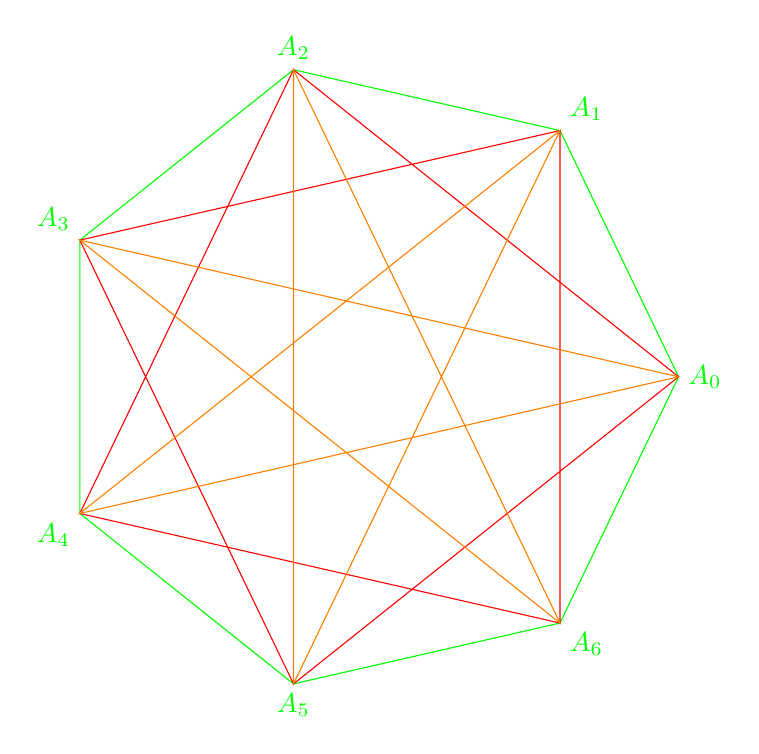
\begin{tikzpicture}
  \draw[color=green]
  (4, 0) node [right]{$A_0$} --
  (2.493959207434934,3.127325929872119) node [above right]{$A_1$} --
  (-0.8900837358252573,3.899711648727294) node[above]{$A_2$}--
  (-3.603875471609676,1.735534956470233) node[above left]{$A_3$}--
  (-3.603875471609676,-1.735534956470232) node[below left]{$A_4$}--
  (-0.8900837358252583,-3.899711648727294) node[below]{$A_5$} --
  (2.493959207434933,-3.127325929872119) node[below right]{$A_6$} --
  cycle;
  \draw[color=red]
  (4, 0) --
  (-0.8900837358252573,3.899711648727294) --
  (-3.603875471609676,-1.735534956470232) --
  (2.493959207434933,-3.127325929872119) --
  (2.493959207434934,3.127325929872119) --
  (-3.603875471609676,1.735534956470233) --
  (-0.8900837358252583,-3.899711648727294) --
  cycle;
  \draw[color=orange]
  (4, 0) --
  (-3.603875471609676,1.735534956470233) --
  (2.493959207434933,-3.127325929872119) --
  (-0.8900837358252573,3.899711648727294) --
  (-0.8900837358252583,-3.899711648727294) --
  (2.493959207434934,3.127325929872119) --
  (-3.603875471609676,-1.735534956470232) --
  cycle;
\end{tikzpicture}
\end{center}

\end{enumerate}

